%--------------------------------------------------------------------------------------
%	PACKAGES AND OTHER DOCUMENT CONFIGURATIONS
%----------------------------------------------------------------------------------------


\documentclass[a4paper,12pt]{article}
\usepackage[english]{babel}
\usepackage[latin1]{inputenc}
\usepackage{amsmath}
\usepackage{amssymb}
\usepackage{amsfonts}
\usepackage{graphicx}
\usepackage[colorinlistoftodos]{todonotes}
\usepackage[toc,page]{appendix}
\usepackage{setspace}
\doublespacing
\usepackage{listings}
\usepackage{booktabs}
\usepackage{geometry}
\usepackage[bottom]{footmisc}
\usepackage{longtable}
% \usepackage[demo]{graphicx}
\usepackage{subfig}
\usepackage{multirow}
\usepackage{tikz}
\usetikzlibrary{fit}
\usetikzlibrary{arrows}
\renewcommand{\arraystretch}{0.7}
\renewcommand{\labelitemi}{$\triangleright$}
 \geometry{
 a4paper,
 total={170mm,257mm},
 left=25mm,
 top=30mm,
 right=25mm,
 bottom=25mm,
 }
 \usepackage{hyperref}
 \hypersetup{
    bookmarks=true,         % show bookmarks bar?
    unicode=false,          % non-Latin characters in Acrobat’s bookmarks
    pdftoolbar=true,        % show Acrobat’s toolbar?
    pdfmenubar=true,        % show Acrobat’s menu?
    pdffitwindow=false,     % window fit to page when opened
    pdfstartview={FitH},    % fits the width of the page to the window
    pdftitle={Design_Report},    % title
    pdfauthor={Jacob Pichelman, Luca Poll},     % author
    pdfsubject={Subject},   % subject of the document
    pdfcreator={Creator},   % creator of the document
    pdfproducer={Producer}, % producer of the document
    pdfkeywords={keyword1, key2, key3}, % list of keywords
    pdfnewwindow=true,      % links in new PDF window
    colorlinks=false,       % false: boxed links; true: colored links
    linkcolor=red,          % color of internal links (change box color with linkbordercolor)
    citecolor=green,        % color of links to bibliography
    filecolor=magenta,      % color of file links
    urlcolor=cyan           % color of external links
}

\definecolor{background}{RGB}{39, 40, 34}
\definecolor{string}{RGB}{230, 219, 116}
\definecolor{comment}{RGB}{117, 113, 94}
\definecolor{normal}{RGB}{248, 248, 242}
\definecolor{identifier}{RGB}{166, 226, 46}

\lstset{
  language = SQL,  % choose the language of the code
  linewidth = 16cm,
  numbers = left, % where to put the line-numbers
  stepnumber=1,  % the step between two line-numbers.        
  numbersep=5pt, % how far the line-numbers are from the code
  numberstyle=\tiny\color{black}\ttfamily,
  backgroundcolor=\color{background}, % choose the background color. You must add \usepackage{color}
  showspaces=false, % show spaces adding particular underscores
  showstringspaces=false,             % underline spaces within strings
  showtabs=false, % show tabs within strings adding particular underscores
  tabsize=4,                          % sets default tabsize to 2 spaces
  captionpos=b,                       % sets the caption-position to bottom
  breaklines=true,                    % sets automatic line breaking
  breakatwhitespace=true, % sets if automatic breaks should only happen at whitespace
  title=\lstname,  % show the filename of files included with \lstinputlisting;
  basicstyle=\color{normal}\ttfamily,     % sets font style for the code
  keywordstyle=\color{magenta}\ttfamily,  % sets color for keywords
  stringstyle=\color{string}\ttfamily,    % sets color for strings
  commentstyle=\color{comment}\ttfamily,  % sets color for comments
  emph={format_string, eff_ana_bf, permute, eff_ana_btr},
  emphstyle=\color{identifier}\ttfamily,
  belowskip=-0.5cm
}


	% biblatex
\usepackage[
       style=authoryear,
       natbib=true,
       maxcitenames=3,
       maxbibnames=11,
       backend=biber,
       pagetracker=page,
       hyperref=true,
       doi=true, 
       mergedate=compact, 
       firstinits=true
    ]{biblatex} 
	\usepackage{csquotes}
	\renewcommand*{\bibsetup}{
		\interlinepenalty=10000\relax % default is 5000
		\widowpenalty=10000\relax
		\clubpenalty=10000\relax
		\raggedbottom
		\frenchspacing
        \biburlsetup}
    \addbibresource{library.bib}

\newcommand{\pic}[1]{%
    \includegraphics[width=6cm]{#1}
}

\begin{document}
\begin{titlepage}

\newcommand{\HRule}{\rule{\linewidth}{0.25mm}} % Defines a new command for the horizontal lines, change thickness here
\setlength{\topmargin}{-0.5in}
\center % Center everything on the page


\includegraphics[scale=0.75]{TSE.png}\\

%----------------------------------------------------------------------------------------
%	HEADING SECTIONS
%----------------------------------------------------------------------------------------
% \\[1.5cm]
\large \textsc{M2 EEE Database Management Systems}
\vspace{1.5cm}
% Name of your heading such as course name
\textsc{\large } % Minor heading such as course title

%----------------------------------------------------------------------------------------
%	TITLE SECTION
%----------------------------------------------------------------------------------------

\HRule \\[0.75cm]
{ \huge \bfseries Observatory of Environmentally-Friendly Companies (OEFC)}\\[0.5cm] % Title of your document
\HRule \\[1.75cm]

%----------------------------------------------------------------------------------------
%	AUTHOR SECTION
%----------------------------------------------------------------------------------------

\large\textsc{Andrew Boomer, \\ Jacob Pichelmann} \\[1.5cm]

%----------------------------------------------------------------------------------------
%	DATE SECTION
%----------------------------------------------------------------------------------------

{\large \today}\\[0.5cm] % Date, change the \today to a set date if you want to be precise

\vfill % Fill the rest of the page with whitespace

\end{titlepage}

%-------------------------------------------------------------
% TABLE OF CONTENTS
\renewcommand{\contentsname}{Table of Contents}
\tableofcontents
\clearpage
%-----------------------------------------------------------------------------

\section{Introduction}
The Covid-19 pandemic direly exposed the fragility of our social and economic system and might serve as a harbinger of what
humanity awaits if we fail to act on the dawning climate crisis.
Acknowledging the urgency of the situation, the Observatory of Environmentally-Friendly Companies (OEFC) aims to promote
green initiatives of companies by establishing a knowledge pool which ultimately serves to promote, monitor and analyze
green actions conducted by companies.
To this end, the OEFC offers a web-based tool which gives an overview of all possible green actions, the companies which
have adopted them and those offering services to support them.
Moreover, the impact of said actions is analyzed by year to year comparison where the measure of success is defined as a reduction in
CO2 emissions.
This paper provides an overview about both the underlying conceptual structure of said tool as well as its technical
implementation.
Additionally, a user guide is provided which allows users to navigate the resulting application effortlessly, regardless
of prior technical know-how.
The paper is hence structured as follows: First, the introduction continues with a description of groups of potential users and
offers a discussion of the universe that is modelled.
Second, an entity relationship model of this universe is introduced.
Third, the entity relationship model is translated into a relational model.
Fourth, having derived all conceptual components, the construction of the database in SQLite is briefly described and the
data sources are outlined.
Fifth, the functionality of the database and the application built on top of it is illustrated by executing a set of queries
and analyses.
Lastly, a user guide explains the few steps necessary to successfully launch and navigate the application.


\subsection{Potential users}
The resulting webtool serves as an informational tool for a wide set of users.
The following groups can be distinguished:
\begin{itemize}
    \item Companies that would like to be aware of green initiatives, plan to invest in environment friendly actions and/or look for examples of such actions and how they could be funded;
    \item Companies that have already invested in such actions and want to communicate about them, and therefore, improve their own reputation;
    \item Consumers who would like to select products or services on the basis of their green quality;
    \item Citizens, notably students, who would like to select companies for a job or an internship, according to their green behavior and reputation.
\end{itemize}

\subsection{Description of the universe to be modelled}

The main agent in this universe is a \textbf{company} which can conduct and support actions, apply for funding and whose
environmental performance is recorded.
In this regard, the following information is registered per year: the quantity of carbon emissions, the turnover, the total amount of
investment in green actions and the number of recruitments related to green actions. \\

\textbf{A company} is known by its name, its main location (city \& country), its website address, its sector (energy, agriculture,
aircraft construction, transport ...), its size, the actions it has carried out, and the type of actions it can support or certify.
Certification consists in guaranteeing with a label the quality or the realization conditions of an action. \\

\textbf{An action type} has:
\begin{itemize}
    \item a category (production, service, internal behavior, external behavior, financing...);
    \item a description (using renewable energy, offsetting of travel emissions, usage of green bonds, phasing out
    of plastic straws, ...);
    \item its main impact (emission reduction, pollution prevention, perseverance of biodiversity ...);
    \item possible public and/or private funding programs to implement that type of actions.
\end{itemize}

\textbf{An action} is implemented a given year by a company, belongs to a type of actions, is certified or not by another company
and may have been funded after applying to funding program(s).
We also record the number of likes received by each action. \\

\textbf{A funding program} is known by its name, a maximum allowable amount by action, its eligible types of actions, a procedure
(text or link towards a web page explaining the procedure) and if it is cumulative or not with other programs.
For each company, each of the granted (funded) actions must be recorded with the corresponding funding program, its year of obtainment and amount.


\section{Entity Relationship Model}
We use an entity relationship (ER) model to graphically represent the universe outlined above.
In a nutshell, the ER model depicts the objects of the universe (entities) and the relations between those objects.
In this context an entity can be anything that can exist independently and can be identified uniquely.
To put this in layman terms, an entity is essentially some aspect of the universe that can be distinguished from other
aspects of the same universe.
Relationships, on the other hand, capture how entities are related to one another.
A relationship is hence an association among two or more entities.
Putting this theoretical definition to work, we first identify the natural entities of the universe given.
We then proceed by modelling the associations between said entities, which build on a set of assumptions that are outlined
in section \ref{sec:assumptions}.
The resulting entity relationship schema is displayed in figure \ref{fig:ER}.
Note that the unique identifier of each entity is \underline{underlined}.
The domain of each attribute is given in the relational model in section \ref{sec:relational}.

\begin{figure}
    \caption{Entity Relationship Model}
    \label{fig:ER}
    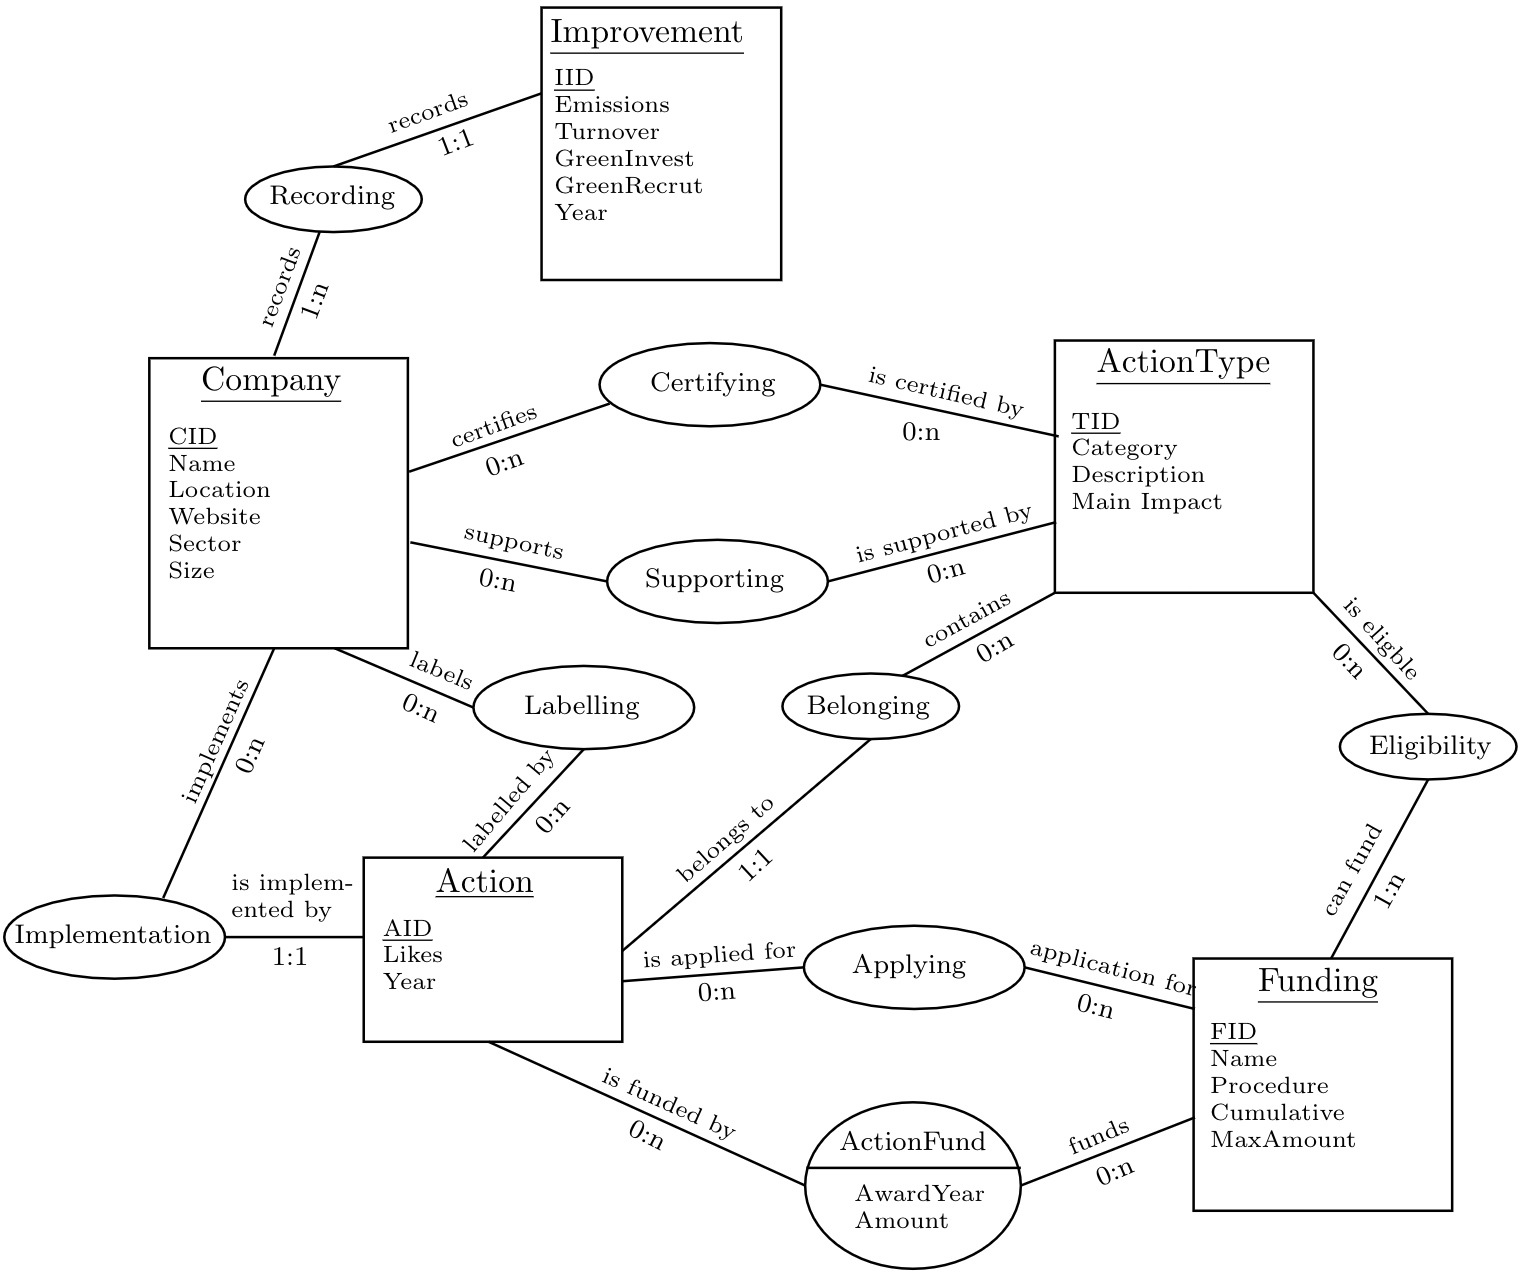
\includegraphics[width=16cm]{ER_model.png}
\end{figure}


\clearpage
\subsection{Assumptions} \label{sec:assumptions}
The associations between entities are modelled based on the following set of assumptions:
\begin{itemize}
    \item Each improvement record corresponds to one and only one company.
    \item Each action belongs to one and only one action type.
    \item The source of likes of an action is not of interest, we only record the amount.
    \item Each funding program must fund at least one action type.
    \item Each company must have at least one record in the improvements table.
    \item One instance of an action is implemented by exactly one company.
\end{itemize}

\subsection{Integrity Constraints}
Additionally, we the inserted data has to pass a set of integrity checks, namely:
\begin{enumerate}
    \item The funding amount must be greater than 0.
    \item The maximum amount per funding program must be greater than 0.
    \item The funded amount cannot be greater than the maximum amount per action of a funding program.
    \item The funded action must be in the set of eligible actions of a funding program.
    \item The label must come from a company who is able to certify the action type the action belongs to.
    \item AwardYear must be less or equal to Action.Year, i.e. an action cannot be funded after it was implemented.
    \item Actions can be funded by multiple funding programs only if all of them are cumulative.
\end{enumerate}

Integrity constraints (3) to (7) are cross-table constraints, which means they require a subquery in order to check whether
the constraint has been violated.
In SQLite, subqueries cannot go into a check constraint, so we had to implement these integrity constraints in a different way.
Our solution for this was to use the "CREATE TRIGGER" function.

For Integrity Constraint (3) this query is:

\begin{lstlisting}[language=SQL]
    CREATE TRIGGER amount_check
    BEFORE INSERT ON ACTIONFUND
    WHEN NEW.AMOUNT > (
    SELECT DISTINCT FUNDING.MAXAMOUNT
    FROM FUNDING, ACTIONFUND
    WHERE FUNDING.FID = ACTIONFUND.FID)
    BEGIN
    SELECT RAISE(FAIL, 'Funded Amount Cannot Be Greater Then Max Amount');
    END;
\end{lstlisting}

For Integrity Constraint (4) this query is:

\begin{lstlisting}[language=SQL]
CREATE TRIGGER aid_check
BEFORE INSERT ON ACTIONFUND
WHEN NEW.FID NOT IN (
SELECT DISTINCT ELIGIBILITY.FID
FROM ACTION, ELIGIBILITY
WHERE ACTION.AID = NEW.AID
AND ACTION.TID = ELIGIBILITY.TID)
BEGIN SELECT RAISE(FAIL, 'Funding Program not in List of Eligible Programs for this Action Type'); END;
\end{lstlisting}

For Integrity Constraint (5) this query is:

\begin{lstlisting}[language=SQL]
    CREATE TRIGGER cert_check
    BEFORE INSERT ON LABELLING
    WHEN NEW.CID NOT IN (
    SELECT DISTINCT CERTIFYING.CID
    FROM ACTION, ACTIONTYPE, CERTIFYING
    WHERE NEW.AID = ACTION.AID
    AND ACTION.TID = CERTIFYING.TID)
    BEGIN
    SELECT RAISE(FAIL, 'Company Cannot Label This Type Of Action');
    END;
\end{lstlisting}

For Integrity Constraint (6) this query is:

\begin{lstlisting}[language=SQL]
CREATE TRIGGER year_check
BEFORE INSERT ON ACTIONFUND
WHEN NEW.AWARDYEAR > (
SELECT DISTINCT ACTION.YEAR
FROM ACTION
WHERE ACTION.AID = NEW.AID)
BEGIN SELECT RAISE(FAIL, 'Funding Award Year Cannot After Action Year');
END;
\end{lstlisting}

For Integrity Constraint (7) this query is:

\begin{lstlisting}[language=SQL]
    CREATE TRIGGER cumulative_check
    BEFORE INSERT ON ACTIONFUND
    WHEN NEW.FID IN (
    SELECT DISTINCT FID
    FROM(
        SELECT 1 as Holder, ACTIONFUND.FID
        FROM ACTIONFUND, FUNDING
        WHERE ACTIONFUND.FID = FUNDING.FID
        AND FUNDING.CUMULATIVE = 'FALSE'
    ) GROUP BY Holder
    HAVING COUNT(FID) > 1)
    BEGIN SELECT RAISE(FAIL, 'Funding Program is Not Cumulative, Cannot Support Multiple Actions');
    END;
\end{lstlisting}

Finally, to ensure there were no unintended integrity constraint conflicts, the \textbf{ActionFund} table was filled last.
If data that does not satisfy the integrity constraints is placed in the source files of the database, the user will
receive and error when trying to fill the database that indicates which constraint was violated.
The faulty data can then be easily changed accordingly.
An example of such an error is shown in figure \ref{fig:integrity}.

\begin{figure}[h!]
    \centering
    \caption{Example of Integrity Constraint Violation}
    \label{fig:integrity}
    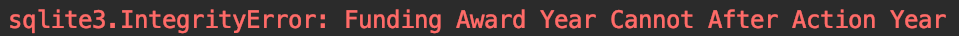
\includegraphics[width=12cm]{Integrity_Violation.png}
\end{figure}



\section{Relational Model} \label{sec:relational}

We can transform the ER model into a relational model by following three steps.
\begin{enumerate}
    \item We start by constructing a table for each entity class, namely \textbf{Improvement, Company, Action, ActionType}
    and \textbf{Funding}.
    The name of the entity becomes the table name, the entity's properties become the table's attributes and finally
    the unique identifier of each entity translates to the primary key of the resulting table.
    \item In the second step we design additional tables for all \textit{many to many} relationships that this ER model
    includes.
    From this procedure we obtain six additional tables: \textbf{Supporting, ActionFund, Applying, Certifying, Labelling}
    and \textbf{Eligibility}.
    The primary keys of these tables are the tuples of their foreign keys, shown in greater detail below.
    Foreign keys are indicated with a star *.
    \item Lastly, we account for the remaining associations by adding them as foreign keys to the existing tables where
    the underlying cardinality is one.
\end{enumerate}

Implementing these steps yields the following relational model:

\begin{itemize}
    \item Action(\underline{AID} : int; Likes : int; Year : int, CID*, TID*)
    \item ActionType(\underline{TID} : int; Category : varchar(100); Description : varchar(500); MainImpact : varchar(100))
    \item Improvement(\underline{IID} : int, Emissions : double; Turnover : double; GreenInvest : double; GreenRecrut : int, Year: int; CID*)
    \item Company(\underline{CID} : int; Name : varchar(100); Location : varchar(100); Website : varchar(100); Sector : varchar(100); Size : double)
    \item Eligibility(\underline{FID*, TID*})
    \item Certifying(\underline{CID*, AID*})
    \item Labelling(\underline{CID*, AID*})
    \item Supporting(\underline{CID*, AID*})
    \item Applying(\underline{FID*, AID*})
    \item ActionFund(\underline{FID*, AID*}; AwardYear : int; Amount : double)
\end{itemize}

\section{Generating and Filling the Database}
The backend of OEFC's webtool runs on an SQLite database which is filled automatically from a Python scraping script.
In the current implementation a google sheet document that contains all collected data is scraped.
However, if there were data sources for all necessary data points, the script could easily be changed to retrieve data
from said sources, e.g. APIs.
This backend implementation hence comprises a lot of flexibility as new data can be inserted easily.
In order to cater to the number of different users with different levels of technical knowledge we additionally built a
desktop application which performs a set of analyses described in greater detail in section \ref{sec:queries}.
Moreover, this application also updates the database with every run meaning that the analysis is always conducted on the
most recent set of data.

\subsection{Companies}

As examples for companies observed by OEFC we chose a set of 11 companies that cover a broad spectrum of business activity
and are situated in different geographical regions.
We include both well established firms such as Volkswagen and Walmart as well as new and disruptive ventures such as Tesla
and Spotify.
Arguably older companies, especially those operating in areas with likely harmful environmental consequences, such as Total SE
and Volkswagen face greater pressure from the public to operate in a way that protects the environment.
We are interested to see how this reflects in both their environmental performance and their actions.

\subsection{Improvement (Environmental Statistics)}
Again, we collected real world data from business and sustainability reports to fill this table meaningfully.
The turnover of each of the companies in our sample is publicly disclosed hence those values can be taken at face value.
The CO2 emissions, however, are often only listed in reports spanning hundreds of pages and are frequently given by source of
emissions, e.g. production or business related travel.
The resulting data is hence an approximation of the total level of CO2 emissions and can be interpreted in relative terms
for one company (over time) but should be taken with a grain of salt when comparing emissions between companies.
Similarly, the data on green investments is not available in an aggregated format, resulting in approximate values taken
from the respective sustainability reports.
Unfortunately there is no public information available on the number of recruitments that resulted from a company's green
actions.
We hence approximated this value by assessing each company's \textit{attractiveness} for individuals looking to employ
their skill set in an environmentally friendly context (e.g. Tesla supporting the shift to electric vehicles and solar
energy is perceived as positive whereas the Diesel scandal led to Volkswagen's reputation being shattered) and set this
in relation to the total number of employees of each company to derive an approximation.

\subsection{Action Types}
We manually collected a set of eight different action types, with we obtain from companies' sustainability reports and
general online press releases.
As this is part of their marketing it was often a challenge to distinguish between companies' goals and their actual
implementation of actions but the resulting data indeed captures past behaviour of firms.
Fortunately many types of actions are taken by different companies which allows for meaningful comparison.

\subsection{Actions}
With a total of 19 actions we succeeded in collecting at least one action for each company and multiple actions for some,
which provides a good basis for analysis.
However, even after consulting the sustainability reports, there was often no indication when a given action was implemented.
The indicated year is hence just an approximation based on the assumption that actions have been implemented shortly before being
communicated in reports and press releases.

\subsection{Labelling, Supporting, Certifying}
After an extensive research endeavour we were unable to find any information on companies supporting, certifying or labelling
specific environmental actions.
The data on these interlinkages is hence based on the company's environmental history.
We were able to research, for instance, that Volkswagen led the initiative of reusing old parts hence we assign it the
capability of supporting and labelling in this area.
Similarly, Spotify early on discussed the significant role of business related air travel, prompting us to give them a
\textit{first mover} status in this context.
It has to be kept in mind, however, that these interlinkages are not derived from actual quantifiable data.

\subsection{Funding Programs}
There is no publicly disclosed information whether or not a company profits from a funding program when implementing a
green action.
We therefore researched on funding programs to then match them to the action types we obtained from the sustainability
reports.
Most such funding programs are provided by the government and in fact intend at supporting small and medium size enterprises
which is at odds with the firms we have in our sample.
The key areas of support are green energy and waste reduction.
Motivated by these observations we manually design five different funding programs which take their inspiration from real government
programs but are in fact completely fictive.

\clearpage
\section{Measuring Companies' Environmental Performance} \label{sec:queries}

We analyze the data through three distinct packages, each consisting out of a set of queries.
Some results are additionally highlighted with figures.
For each set we show the required information and the query that was implemented to obtain said information.
In some instances additional remarks are noted.

\subsection{Package 1: Making companies aware of green initiatives by sector}

\begin{table}[!htb]
    \caption{Query F1 - F1.5}
    --------------------------------------------------------------------------------
\\Showcase functionality of view F1.\\
--------------------------------------------------------------------------------
\begin{lstlisting}[language = SQL]
SELECT * FROM ActionsInTechnology
\end{lstlisting}
--------------------------------------------------------------------------------\\\begin{tabular}{rlr}
\toprule
   CID & Name     &   AID \\
\midrule
     3 & Apple    &     1 \\
     1 & Alphabet &     4 \\
     3 & Apple    &     8 \\
     3 & Apple    &     9 \\
    10 & Snapchat &    12 \\
    11 & Spotify  &    13 \\
    11 & Spotify  &    17 \\
\bottomrule
\end{tabular} \\
    Remark F1: We only show the resulting view, the underlying SQL code to produce this view can be seen when using  the
    desktop application.
    As the view serves to display the companies of a \textit{given} sector, we allow the user to make a choice on the
sector, when using the app.
There is hence great flexibility accounting for different user interests.
In the example displayed in this report \textit{Technology} has been chosen.
\end{table}



\begin{table}[!htb]
    \caption{Query R1}
    --------------------------------------------------------------------------------
\\Information about the evolution through time of companies of a given sector.\\
--------------------------------------------------------------------------------
\begin{lstlisting}[language = SQL]
SELECT IMPROVEMENT.*, COMPANY.NAME
FROM COMPANY, IMPROVEMENT 
WHERE COMPANY.CID = IMPROVEMENT.CID
AND COMPANY.SECTOR = 'Technology'
\end{lstlisting}
--------------------------------------------------------------------------------\\\begin{tabular}{rrrrrrrl}
\toprule
   IID &       Emissions &   Turnover &   GreenInvest &   GreenRecruit &   CID &   Year & Name     \\
\midrule
     1 &     3.29491e+06 &     110855 &          4000 &           1200 &     1 &   2017 & Alphabet \\
     2 &     1.50272e+07 &     136819 &          3700 &           8000 &     1 &   2018 & Alphabet \\
     3 &     8.57655e+06 &     161857 &          6500 &           8430 &     1 &   2019 & Alphabet \\
     7 &     2.71e+07    &     247510 &           423 &          12000 &     3 &   2017 & Apple    \\
     8 &     2.46e+07    &     260170 &           530 &          14230 &     3 &   2018 & Apple    \\
     9 &     2.41e+07    &     265600 &           588 &          17400 &     3 &   2019 & Apple    \\
    28 & 50000           &        825 &             5 &              0 &    10 &   2017 & Snapchat \\
    29 & 43000           &       1180 &             7 &             20 &    10 &   2018 & Snapchat \\
    30 & 38000           &       1716 &            10 &             70 &    10 &   2019 & Snapchat \\
    31 & 15000           &       1200 &           125 &              5 &    11 &   2017 & Spotify  \\
    32 & 18000           &       4320 &           120 &             12 &    11 &   2018 & Spotify  \\
    33 & 19400           &       6760 &           194 &             25 &    11 &   2019 & Spotify  \\
\bottomrule
\end{tabular} \\
    Remark R1: Similar to the prior query the user is again presented with the choice of sector.
Again we chose \textit{Technology} as an example.
\end{table}



\begin{table}[!htb]
    \caption{Query R2}
    --------------------------------------------------------------------------------
\\Number of granted (funded) actions and the total amount of grants received by sector. Limit to sectors having received more than X grants and sort according to the amount. Give also a graphic representation of the answer.\\
--------------------------------------------------------------------------------
\begin{lstlisting}[language = SQL]
SELECT COMPANY.SECTOR,
	COUNT(ACTIONFUND.FID) As GrantedActions, 
	SUM(ACTIONFUND.Amount) as TotalAmount 
FROM COMPANY, ACTION, ACTIONFUND 
WHERE COMPANY.CID = ACTION.CID 
AND ACTION.AID = ACTIONFUND.AID 
GROUP BY COMPANY.SECTOR 
HAVING GrantedActions > 0 
ORDER BY TotalAmount DESC
\end{lstlisting}
--------------------------------------------------------------------------------
\\\begin{tabular}{lrr}
\toprule
 Sector          &   GrantedActions &   TotalAmount \\
\midrule
 Technology      &                3 &         79000 \\
 CarManufacturer &                1 &         33000 \\
 Food\&Bev        &                2 &         18000 \\
 Retail          &                1 &         12000 \\
\bottomrule
\end{tabular} \\
    Remark R2: As funding is scarce, we limit the query to sectors having received more than 0 grants.
However, this could (and should) be changed when more data is available.
\end{table}

\begin{figure}[h!]
    \centering
    \caption{Query R2}
    \label{fig:R2}
    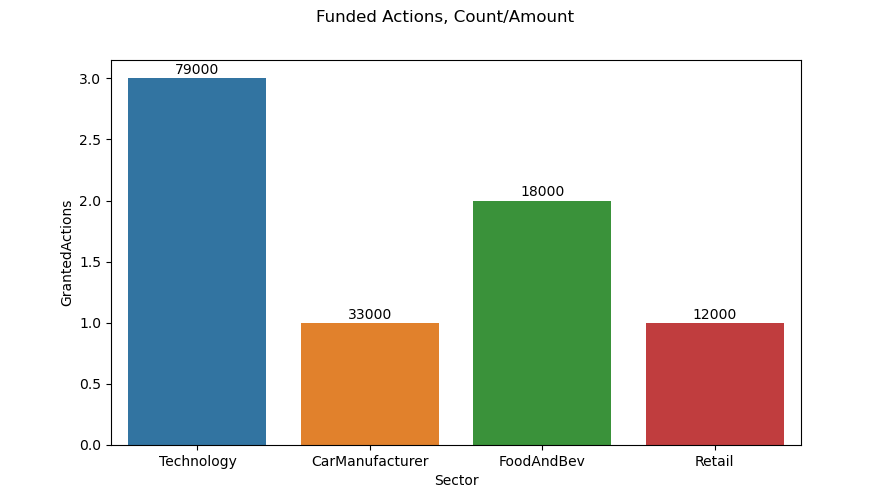
\includegraphics[width=16cm]{R2_plot.png}
\end{figure}



\begin{table}[!htb]
    \caption{Query R3}
    --------------------------------------------------------------------------------
\\For each type of actions display the companies that can help for its realization.\\
--------------------------------------------------------------------------------
\begin{lstlisting}[language = SQL]
SELECT ACTIONTYPE.TID, ACTIONTYPE.DESCRIPTION,
	COMPANY.CID, COMPANY.NAME 
FROM ACTIONTYPE, CERTIFYING, COMPANY 
WHERE COMPANY.CID = CERTIFYING.CID 
AND ACTIONTYPE.TID = CERTIFYING.TID
\end{lstlisting}
--------------------------------------------------------------------------------
\\\begin{tabular}{rlrl}
\toprule
   TID & Description                                  &   CID & NAME       \\
\midrule
     1 & Usage of renewable energy                    &     7 & Siemens    \\
     4 & Set up of charging stations of electric cars &     8 & Tesla      \\
     5 & Reusage of old components                    &     5 & Volkswagen \\
     7 & Offsetting of travel emissions               &    11 & Spotify    \\
     1 & Usage of renewable energy                    &     8 & Tesla      \\
     1 & Usage of renewable energy                    &     5 & Volkswagen \\
\bottomrule
\end{tabular}
\end{table}

\begin{table}[!htb]
    \caption{Query R4}
    --------------------------------------------------------------------------------
\\Number of companies by location. Give a world map chart (import in excel the data..., look for a tutorial about that).\\
--------------------------------------------------------------------------------
\begin{lstlisting}[language = SQL]
SELECT Country, COUNT(CID) as NumCompanies 
FROM COMPANY 
GROUP BY Country
ORDER BY NumCompanies DESC
\end{lstlisting}
--------------------------------------------------------------------------------
\\\begin{tabular}{lr}
\toprule
 Location                 &   NumCompanies \\
\midrule
 United States of America &              6 \\
 Germany                  &              2 \\
 France                   &              2 \\
 Sweden                   &              1 \\
\bottomrule
\end{tabular}
\end{table}

\begin{figure}[h!]
    \centering
    \caption{Query R4}
    \label{fig:R4}
    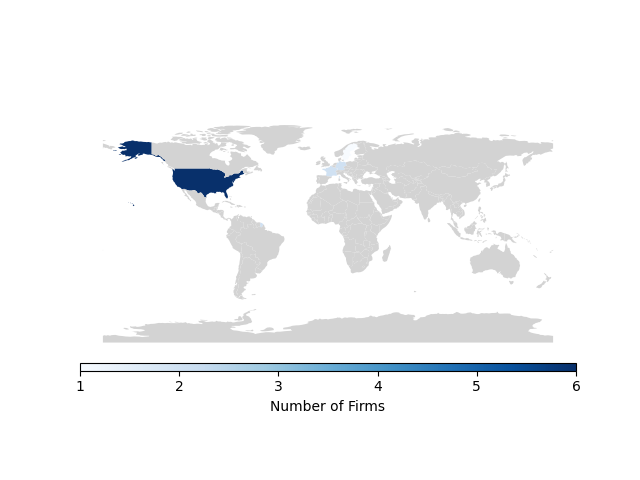
\includegraphics[width=16cm]{R4_plot.png}
\end{figure}

\clearpage
\newpage

\subsection{Package 2: Reputation and evolution of analysis of companies}
\begin{table}[!htb]
    \caption{Query R5}
	--------------------------------------------------------------------------------
\\Companies in the decreasing order of the total number of likes they got through their actions.\\
--------------------------------------------------------------------------------
\begin{lstlisting}[language = SQL]
SELECT COMPANY.CID, COMPANY.Name, 
	SUM(ACTION.Likes) AS NumLikes 
FROM ACTION, COMPANY 
WHERE ACTION.CID = COMPANY.CID 
GROUP BY COMPANY.Name 
ORDER BY NumLikes DESC
\end{lstlisting}
--------------------------------------------------------------------------------
\\\begin{tabular}{rlr}
\toprule
   CID & Name       &   NumLikes \\
\midrule
     8 & Tesla      &    1877000 \\
    10 & Snapchat   &    1430000 \\
     3 & Apple      &    1230000 \\
    11 & Spotify    &    1070000 \\
     2 & Starbucks  &     650000 \\
     6 & Walmart    &     162000 \\
     1 & Alphabet   &     120000 \\
     5 & Volkswagen &      98000 \\
     4 & Airbus     &      32000 \\
     9 & Total SE   &      12000 \\
     7 & Siemens    &      11300 \\
\bottomrule
\end{tabular}
\end{table}

\begin{table}[!htb]
    \caption{Query R6}
	--------------------------------------------------------------------------------
\\The company that got the most number of certified actions.\\
--------------------------------------------------------------------------------
\begin{lstlisting}[language = SQL]
SELECT COMPANY.CID, COMPANY.Name, 
COUNT(LABELLING.AID) as NumCerts 
FROM COMPANY, LABELLING, ACTION
WHERE COMPANY.CID = ACTION.CID AND
LABELLING.AID = ACTION.AID 
GROUP BY COMPANY.CID, COMPANY.Name
ORDER BY NumCerts DESC LIMIT 3
\end{lstlisting}
--------------------------------------------------------------------------------
\\\begin{tabular}{rlr}
\toprule
   CID & Name    &   NumCerts \\
\midrule
     6 & Walmart &          2 \\
     4 & Airbus  &          1 \\
     8 & Tesla   &          1 \\
\bottomrule
\end{tabular} \\
    Remark R6: We limit the output to the top 3 observations instead of just showing the top one, as it might happen that
companies have the same number of certified actions, which is indeed the case in our data.
\end{table}



\begin{table}[!htb]
    \caption{Query R7}
	--------------------------------------------------------------------------------
\\Companies that propose help and also provide certifications.\\
--------------------------------------------------------------------------------
\begin{lstlisting}[language = SQL]
SELECT DISTINCT comb.CID, COMPANY.Name
FROM(
	SELECT DISTINCT CID
	FROM SUPPORTING 

	UNION ALL 

	SELECT DISTINCT CID
	FROM CERTIFYING
) comb, COMPANY
WHERE comb.CID = COMPANY.CID
\end{lstlisting}
--------------------------------------------------------------------------------
\\\begin{tabular}{rl}
\toprule
   CID & Name       \\
\midrule
     3 & Apple      \\
     5 & Volkswagen \\
     8 & Tesla      \\
    11 & Spotify    \\
     7 & Siemens    \\
\bottomrule
\end{tabular}
\end{table}

\begin{table}[!htb]
    \caption{Query R8}
	--------------------------------------------------------------------------------
\\Companies whose green situation has been improved between two given years: the quantity of carbon emissions decreases.\\
--------------------------------------------------------------------------------
\begin{lstlisting}[language = SQL]
SELECT COMPANY.CID, COMPANY.Name, 
	sum(Emissions) filter(where Year = 2018) - sum(Emissions) filter(where Year = 2017) Diff20182017,
	sum(Emissions) filter(where Year = 2019) - sum(Emissions) filter(where Year = 2018) Diff20192018 
FROM COMPANY, IMPROVEMENT 
WHERE COMPANY.CID = IMPROVEMENT.CID 
GROUP BY COMPANY.CID 
HAVING Diff20182017 < 0 OR Diff20192018 < 0
\end{lstlisting}
--------------------------------------------------------------------------------
\\\begin{tabular}{rlrr}
\toprule
   CID & Name       &   Diff\_2018\_2017 &    Diff\_2019\_2018 \\
\midrule
     1 & Alphabet   &      1.17323e+07 &      -6.45067e+06 \\
     2 & Starbucks  &  61000           & -325000           \\
     3 & Apple      &     -2.5e+06     & -500000           \\
     4 & Airbus     & 310000           & -680000           \\
     5 & Volkswagen & 160000           &      -1.6e+06     \\
     6 & Walmart    &     -1.154e+06   & -120000           \\
     7 & Siemens    &     -2.001e+06   & -160000           \\
     9 & Total SE   &     -2.5e+06     &      -1.9e+06     \\
    10 & Snapchat   &  -7000           &   -5000           \\
\bottomrule
\end{tabular} \\
    Remark R8: We track environmental data of companies between 2017 and 2019.
We can therefore check two pairs of years and see if the company's environmental situation has improved from one year to
another.
Interestingly we find that for some companies (Starbucks, Airbus, Volkswagen) the situation did not improve between 2017
and 2018 but then they were able to turn it around and indeed improved between 2018 and 2019.
We would not have been able to spot this development if we would have analyzed only two years.
Moreover, we find that the situation got worse over time for Tesla and Spotify, as they are not displayed in the query result.
This can, however, be attributed to the fact that these are both strong growth companies where a rise in emissions mainly
stems from a significant increase in business activity.
\end{table}



\clearpage
\newpage
\subsection{Package 3: Analysis of the funding programs}

\begin{table}[!htb]
    \caption{Query F2 - F2.5}
    --------------------------------------------------------------------------------
\\Showcase functionality of view F2.\\
--------------------------------------------------------------------------------
\begin{lstlisting}[language = SQL]
SELECT * FROM EligibleTypes
\end{lstlisting}
--------------------------------------------------------------------------------
\\\begin{tabular}{rlrl}
\toprule
   FID & Name                    &   TID & Description                                  \\
\midrule
     1 & Clean Energy for All    &     1 & Usage of renewable energy                    \\
     2 & Clean Ocean Initiative  &     2 & Phasing out of plastic straws                \\
     3 & Waste Reduction Program &     2 & Phasing out of plastic straws                \\
     4 & Fly Green               &     7 & Offsetting of travel emissions               \\
     5 & Recycling Rocks!        &     5 & Reusage of old components                    \\
     1 & Clean Energy for All    &     4 & Set up of charging stations of electric cars \\
\bottomrule
\end{tabular} \\
    Remark F2: We again only show the resulting view.
    The underlying SQL code to construct this view can be seen when
    using the desktop application.
\end{table}

\begin{table}[!htb]
    \caption{Query R9}
	--------------------------------------------------------------------------------
\\Evolution of the investment of a given company per year: number of recruitments, the percentage of green investment compared to the amount of turnover. Give also a graphic representation.\\
--------------------------------------------------------------------------------
\begin{lstlisting}[language = SQL]
SELECT COMPANY.CID, COMPANY.Name, Year,
	GreenRecruit, GreenInvest, Turnover, 
	(GreenInvest/Turnover)*100 AS GreenInvestPercentage
FROM COMPANY, IMPROVEMENT 
WHERE COMPANY.CID = IMPROVEMENT.CID
AND COMPANY.NAME = 'Alphabet'
\end{lstlisting}
--------------------------------------------------------------------------------\\\begin{tabular}{rlrrrrr}
\toprule
   CID & Name     &   Year &   GreenRecruit &   GreenInvest &   Turnover &   GreenInvestPercentage \\
\midrule
     1 & Alphabet &   2017 &           1200 &          4000 &     110855 &                 3.60832 \\
     1 & Alphabet &   2018 &           8000 &          3700 &     136819 &                 2.7043  \\
     1 & Alphabet &   2019 &           8430 &          6500 &     161857 &                 4.01589 \\
\bottomrule
\end{tabular} \\
    Remark R9: As in Query F1 and R1 we again let the user choose which company to analyze.
For this report we chose \textit{Alphabet} as an example.
\end{table}



\begin{figure}[h!]
    \centering
    \caption{Query R9}
    \label{fig:R9}
    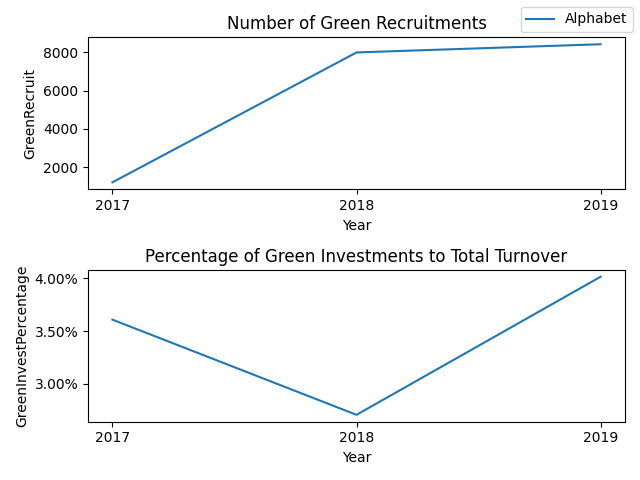
\includegraphics[width=16cm]{R9_plot.png}
\end{figure}

\begin{table}[!htb]
    \caption{Query R10}
	--------------------------------------------------------------------------------
\\Average, max and min amounts of grants and number of grants attributed by each Funding program.\\
--------------------------------------------------------------------------------
\begin{lstlisting}[language = SQL]
SELECT FUNDING.FID, 
	AVG(ACTIONFUND.Amount) as AvgAmount, 
	MAX(ACTIONFUND.Amount) as MaxAmount, 
	MIN(ACTIONFUND.Amount) as MinAmount, 
	COUNT(ACTIONFUND.AID) as NumGrants 
FROM FUNDING, ACTIONFUND 
WHERE FUNDING.FID = ACTIONFUND.FID 
GROUP BY FUNDING.FID
\end{lstlisting}
--------------------------------------------------------------------------------
\\\begin{tabular}{rrrrr}
\toprule
   FID &   AvgAmount &   MaxAmount &   MinAmount &   NumGrants \\
\midrule
     1 &       23000 &       34000 &       12000 &           2 \\
     2 &       10000 &       10000 &       10000 &           1 \\
     3 &        8000 &        8000 &        8000 &           1 \\
     4 &        5000 &        5000 &        5000 &           1 \\
     5 &       36500 &       40000 &       33000 &           2 \\
\bottomrule
\end{tabular}
\end{table}

\begin{table}[!htb]
    \caption{Query R11}
	--------------------------------------------------------------------------------
\\Types of actions without funding program.\\
--------------------------------------------------------------------------------
\begin{lstlisting}[language = SQL]
SELECT ACTIONTYPE.TID, ACTIONTYPE.DESCRIPTION
FROM ACTIONTYPE 
WHERE ACTIONTYPE.TID NOT IN(
SELECT ACTION.TID FROM
ACTION, ACTIONFUND
WHERE ACTION.AID = ACTIONFUND.AID)
\end{lstlisting}
--------------------------------------------------------------------------------
\\\begin{tabular}{rl}
\toprule
   TID & Description                                          \\
\midrule
     3 & Usage of green bonds                                 \\
     6 & Management remuneration based on CO2 emission levels \\
     8 & Supporting biodiversity                              \\
\bottomrule
\end{tabular} \\
    Remark R11: We interpret this OEFC request as checking which implemented actions belong to types that for which no funding
program is available.
Another interpretation would be to check which types of actions are not eligible for funding, but this can be easily derived
from the \textbf{Eligibility} table.
\end{table}



\begin{table}[!htb]
    \caption{Query R12}
	--------------------------------------------------------------------------------
\\Evolution by year of the total amount received by granted actions. Draw also a graphic.\\
--------------------------------------------------------------------------------
\begin{lstlisting}[language = SQL]
SELECT AwardYear, SUM(Amount) as YearlyAmt 
FROM ACTIONFUND 
GROUP BY AwardYear
\end{lstlisting}
--------------------------------------------------------------------------------
\\\begin{tabular}{rr}
\toprule
   AwardYear &   YearlyAmt \\
\midrule
        2017 &       33000 \\
        2018 &       40000 \\
        2019 &       51000 \\
        2020 &       18000 \\
\bottomrule
\end{tabular}
\end{table}

\begin{figure}[!htb]
    \centering
    \caption{Query R12}
    \label{fig:R12}
    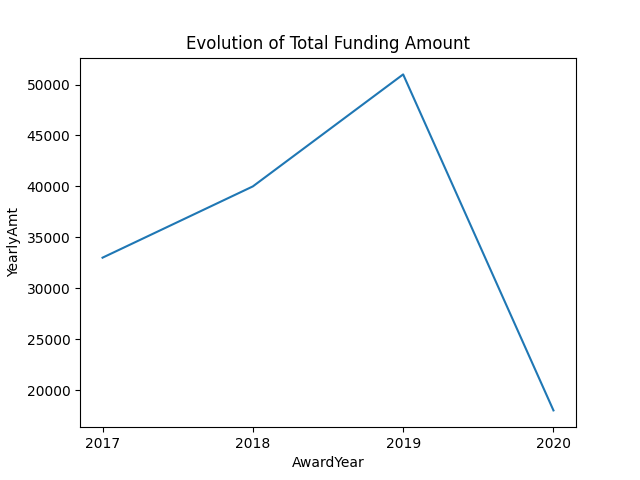
\includegraphics[width=16cm]{R12_plot.png}
\end{figure}

\begin{table}[!htb]
    \caption{Query R13}
	--------------------------------------------------------------------------------
\\Percentage of actions that were funded.\\
--------------------------------------------------------------------------------
\begin{lstlisting}[language = SQL]
SELECT 100 * CAST(Funded AS DECIMAL) / CAST(AllActions AS DECIMAL) as PctFunded 
FROM(
	SELECT 1 As Holder, COUNT(AID) As Funded 
	FROM ACTIONFUND 
	GROUP BY Holder
) AS left 
JOIN (
	SELECT 1 As Holder, COUNT(AID) As AllActions 
	FROM ACTION 
	GROUP BY Holder
) AS right 
ON left.Holder = right.Holder
\end{lstlisting}
--------------------------------------------------------------------------------
\\\begin{tabular}{r}
\toprule
   PctFunded \\
\midrule
          36 \\
\bottomrule
\end{tabular}
\end{table}

\clearpage
\newpage

\subsection{Forecasting future number of actions}
To forecast the future number of actions, we built a time series model which takes in data from the previous year to make forecasts.
Our model is of the form:

\[Actions_{t} = \alpha Actions_{t - 1} + \beta Likes_{t - 1} + \delta Size_{t-1} + \epsilon_{t}\]

From this, a vector of $\begin{pmatrix} Actions_{t}, Likes_{t}, Size_{t}\end{pmatrix}$ can be used to predict $Actions_{t + 1}$.
The underlying rationale is that the past number of actions, as well as their perception by the public (likes) and the
company's size (i.e. their power and resources) are suitable determinants of the future number of actions.

The query to gather the data for this forecast, as well as the forecast plot are shown in Table \ref{OpenTable} and Figure \ref{OpenPlot}.
We expect the number of actions to increase to 13 in 2021.
This is, however, only a tentative forecast, given the limited number of data points.

\begin{table}[!htb]
    \caption{Forecasting the Number of Future Actions}
    \label{OpenTable}
    --------------------------------------------------------------------------------
\\Taking all the necessary assumptions and using the tools of your choice (R, Python...) combined with SQL, try to forecast how the number of actions will evolve in the future\\
--------------------------------------------------------------------------------
\begin{lstlisting}[language = SQL]
SELECT ACTION.YEAR, AVG(COMPANY.SIZE) as Size,
    SUM(ACTION.LIKES) as NumLikes,
    COUNT(ACTION.AID) as NumActions
FROM COMPANY, ACTION
WHERE COMPANY.CID = ACTION.CID
GROUP BY ACTION.YEAR

NumActions(t) = A*Size(t-1) + B*NumLikes(t-1) + C*NumActions(t-1)
        
\end{lstlisting}
--------------------------------------------------------------------------------
\\\begin{tabular}{rrr}
\toprule
    &   Year &   Prediction \\
\midrule
  0 &   2018 &            3 \\
  1 &   2019 &            8 \\
  2 &   2020 &            8 \\
  0 &   2021 &           13 \\
\bottomrule
\end{tabular}
\end{table}

\begin{figure}[!htb]
    \caption{}
    \label{OpenPlot}
\begin{center}
    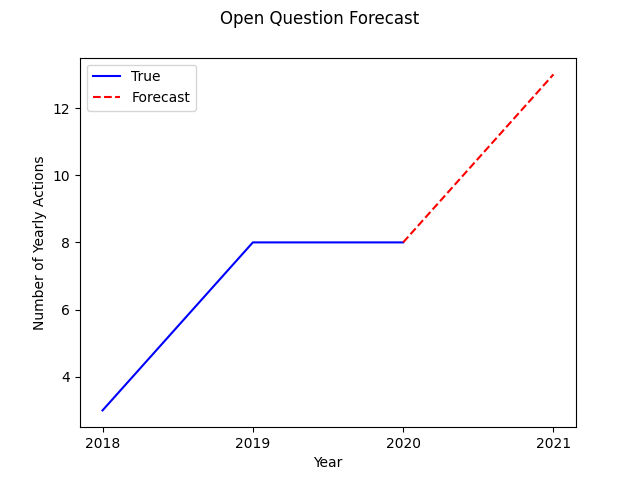
\includegraphics[width=12cm, height=10cm]{Open_plot.png}
\end{center}
\end{figure}

\clearpage
\newpage

\section{User Guide}

In order to cater to the needs of different users we constructed a desktop app running on Python that allows to navigate
analysis.
We built a graphical user interface (GUI) based on the Python package Tkinter to offer a user-friendly way to interact
with the database.
To start the app the following steps have to be followed:
\begin{enumerate}
    \item Unzip the compressed file.
    \item Open Terminal on Mac or Command Prompt on Windows.
 	\item Navigate to the "Code" folder within the unzipped file using Terminal or Command Prompt.
 	\item Run the App.py file using your python executable.
    Depending on your python configuration, this could be "python App.py", "python3 App.py", or "python -m run App.py".
 	\item The code uses the Python Install Packages (pip) library to download any needed packages that are not currently
    installed on the user's machine.
 	\item If the app is accidentally closed before intended, the user is advised to redo Step 4 in Terminal or Command Prompt to restart the App.
\end{enumerate}

Alternatively, the app can of course also be executed from the user's python editor of choice.
Examples of the app's functionality are displayed in figure \ref{fig:app}. \\
\hfill \\

\begin{figure}
   \centering
   \caption{Desktop App Functionality}
\label{fig:app}
\begin{tabular}{cc}
    \pic{Filling.png} &  \pic{Choice.png} \\
    Filling the DB 1 & Making a Choice \\
    \pic{QueryRes.png} &  \pic{Plot.png} \\
    Query Results & Generating a Plot
\end{tabular}
\end{figure}

Once the app is up and running the navigation is very intuitive.
The queries can be executed sequentially and each result can be exported to LaTeX.
Additionally, for some queries there is the option to visualize the result.
The resulting plot is then displayed in the app and will be automatically saved to the output folder.
Note that this app re-fills the database with the most recent data in the google sheet for each run.
It hence inserts the data into a SQLite database that is empty prior to executing the app. \\
\hfill \\
More technically versatile users can also access the SQLite data base directly and make use of the generated views and
stored queries.
To this end we saved the filled database with all data points and executed queries in the data folder under the name
\textit{FilledDB.db}.


\section*{Data Sources}

Airbus: \url{https://www.airbus.com/company/sustainability/reporting-and-performance-data.html} \\
Alphabet: \url{https://www.gstatic.com/gumdrop/sustainability/google-2019-environmental-report.pdf} \\
Apple: \url{https://www.apple.com/environment/pdf/Apple_Environmental_Responsibility_Report_2019.pdf} \\
Siemens: \url{https://assets.new.siemens.com/siemens/assets/api/uuid:16c327d3-3e02-427e-952f-e7f610d954fe/siemens-sustainability-information-2019.pdf} \\
Snapchat: \url{https://citizen.snap.com/products} \\
Spotify: \url{http://q4live.s22.clientfiles.s3-website-us-east-1.amazonaws.com/540910603/files/doc_downloads/govDocs/2019/03/2018-Spotify-Sustainability-Report-FINAL.pdf} \\
Starbucks: \url{https://www.starbucks.com/responsibility/global-report} \\
Tesla: \url{https://www.tesla.com/ns_videos/2019-tesla-impact-report.pdf} \\
Total SE: \url{https://www.sustainable-performance.total.com/en/reporting/our-csr-reports} \\
Volkswagen: \url{https://www.volkswagenag.com/de/sustainability/reporting.html} \\
Walmart: \url{https://corporate.walmart.com/global-responsibility/sustainability/} \\

\end{document}